	\begin{myprops}
	\begin{itemize}
		\iftoggle{eleve}{%
			\item Si des points \hrulefill
			
			\vspace*{0.2cm}
			\hrulefill
			
			\item Si deux segments \hrulefill
			
			\vspace*{0.2cm}
			\hrulefill
			
%			\item Si deux angles \hrulefill
%			
%			\vspace*{0.2cm}
%			\hrulefill
			
			\item Si deux cercles \hrulefill
			
			\vspace*{0.2cm}
			\hrulefill
			
			\vspace*{0.2cm}
			\hrulefill
		}{%
			\item Si des points sont alignés, alors leurs symétriques par rapport à une droite sont \kw{aussi alignés}.
			\item Si deux segments sont symétriques par rapport à une droite, alors ils ont la \kw{même longueur}.
			%\item Si deux angles sont symétriques par rapport à une droite, alors ils ont la \kw{même mesure}.
			\item Si deux cercles sont symétriques par rapport à une droite, alors ils ont le \kw{même rayon} et leurs \kw{centres sont symétriques}.
		}			
	\end{itemize}
	
\end{myprops}


\begin{myexs}
	\begin{itemize}
		\iftoggle{eleve}{%
			\item Le symétrique de \hrulefill
		}{%
			\item Le symétrique de la droite $(d_1)$ par rapport à $(d)$ est la droite $(d_2)$.
		}
		
		\begin{center}
			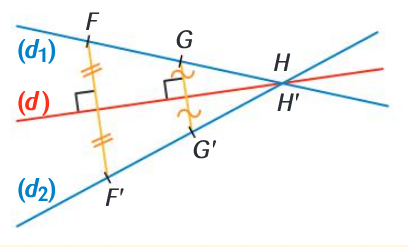
\includegraphics[scale=0.6]{prop1}
		\end{center}
		
		\iftoggle{eleve}{%
			\item $[IJ]$ et $[I'J']$ \hrulefill
		}{%
			\item $[IJ]$ et $[I'J']$ sont symétriques par rapport à la droite $(d)$, donc $IJ = I'J'$.
		}
		
		\begin{center}
			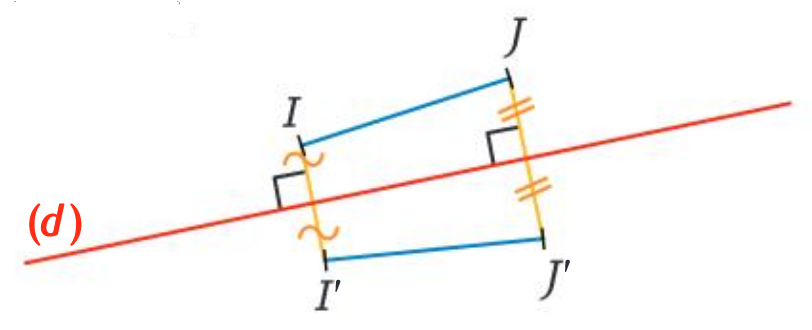
\includegraphics[scale=0.4]{prop2}
		\end{center}
		
		
		\item %$O'$ est le symétrique de $O$ par rapport à la droite $(d)$. 
		\iftoggle{eleve}{%
			Le symétrique du cercle \hrulefill
			
			\vspace*{0.2cm}
			
			\hrulefill
		}{%
			Le symétrique du cercle de centre $O$ et de rayon $r$ est le cercle de centre $O'$ et de rayon $r$.
		}
		\begin{center}
			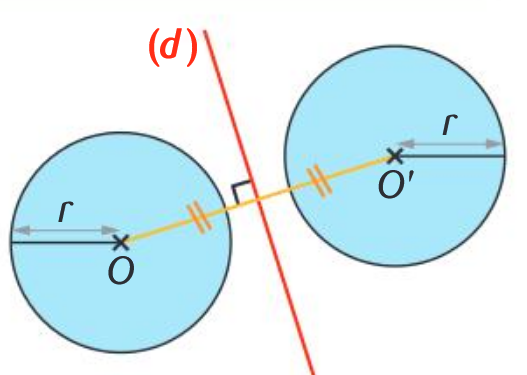
\includegraphics[scale=0.4]{prop3}
		\end{center}
	\end{itemize}
\end{myexs}